\section{Asymptotic behaviour\\\small{The limiting distribution}}
  \begin{frame}{LIMITING DISTRIBUTION}
    \centering
    Evolution for $t$ time steps\\\medskip
    $\downarrow$\\\medskip
    \large \textbf{Does the distribution converge as $\mathbf{t \rightarrow \infty}$?}\\\medskip \small If it does, then the resulting distribution is called \medskip
    \\\medskip
    \Large
    \MakeUppercase{\alert{Limiting distribution}}\\\medskip
    $\downarrow$\\\medskip
    \normalsize
    Concept of \alert{equilibrium}
  \end{frame}

  \begin{frame}
    \centering\Large
    \textsc{How to find the limiting distribution?}\\
    \vspace{30pt}
    \only<2>{\alert{Theory of Markov chains}}
  \end{frame}

  \begin{frame}{LIMITING DISTRIBUTION}
    \centering
      \vspace{30pt}
      \textsc{under some conditions}

      \vspace{10pt}
      \Large
      \textsc{\alert{the limiting distribution is the result of an eigenvalue problem}}
  \end{frame}
\begin{frame}{Asymptotic limit of the Ehrenfest chain}
    \Large 
    \centering
    \vspace{20pt}
    The limiting distribution of the Ehrenfest chain:\\
    \vspace{30pt}
    \textsc{\alert{binomial distribution}}\\
    \vspace{30pt}
    \normalsize
    with trial parameter \alert{$N$} and success probability \alert{$1/2$}
  \end{frame}
  
  \begin{frame}{Asymptotic limit of the Ehrenfest chain}
    \vspace{30pt}
    Example with $N = 10$
    \begin{figure}
      \includegraphics[scale = 0.5]{pictures/binomial.pdf}
    \end{figure}
  \end{frame}

  \section{Asymptotic behaviour\\\small{Mean Recurrence Time}}
  \begin{frame}{Mean Recurrence Time}
    \begin{center}
      \Large \textbf{Mean recurrence time}
    \end{center}
    \alert<3>{At equilibrium}

    Given a certain state, e.\,g.

    \begin{figure}
      


\tikzset{every picture/.style={line width=0.75pt}} %set default line width to 0.75pt        

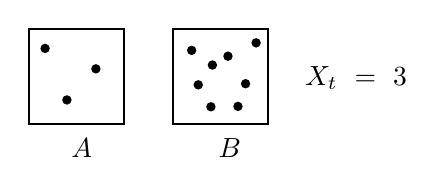
\begin{tikzpicture}[x=0.35pt,y=0.35pt,yscale=-1,xscale=1]
%uncomment if require: \path (0,928); %set diagram left start at 0, and has height of 928

%Shape: Square [id:dp9704491284322827] 
\draw  [color={rgb, 255:red, 0; green, 0; blue, 0 }  ,draw opacity=1 ] (185.93,89.16) -- (284.28,89.16) -- (284.28,187.5) -- (185.93,187.5) -- cycle ;
%Shape: Square [id:dp03136999448950761] 
\draw   (334.93,89.16) -- (433.28,89.16) -- (433.28,187.5) -- (334.93,187.5) -- cycle ;
%Shape: Circle [id:dp7080864036358405] 
\draw  [fill={rgb, 255:red, 0; green, 0; blue, 0 }  ,fill opacity=1 ] (199.13,109.5) .. controls (199.13,107.46) and (200.79,105.8) .. (202.83,105.8) .. controls (204.88,105.8) and (206.53,107.46) .. (206.53,109.5) .. controls (206.53,111.55) and (204.88,113.21) .. (202.83,113.21) .. controls (200.79,113.21) and (199.13,111.55) .. (199.13,109.5) -- cycle ;
%Shape: Circle [id:dp47838494517380514] 
\draw  [fill={rgb, 255:red, 0; green, 0; blue, 0 }  ,fill opacity=1 ] (350.46,111.5) .. controls (350.46,109.46) and (352.12,107.8) .. (354.16,107.8) .. controls (356.21,107.8) and (357.87,109.46) .. (357.87,111.5) .. controls (357.87,113.55) and (356.21,115.21) .. (354.16,115.21) .. controls (352.12,115.21) and (350.46,113.55) .. (350.46,111.5) -- cycle ;
%Shape: Circle [id:dp7883825334163144] 
\draw  [fill={rgb, 255:red, 0; green, 0; blue, 0 }  ,fill opacity=1 ] (416.99,103.77) .. controls (416.99,101.72) and (418.65,100.07) .. (420.7,100.07) .. controls (422.74,100.07) and (424.4,101.72) .. (424.4,103.77) .. controls (424.4,105.81) and (422.74,107.47) .. (420.7,107.47) .. controls (418.65,107.47) and (416.99,105.81) .. (416.99,103.77) -- cycle ;
%Shape: Circle [id:dp9074461888124206] 
\draw  [fill={rgb, 255:red, 0; green, 0; blue, 0 }  ,fill opacity=1 ] (221.66,162.7) .. controls (221.66,160.66) and (223.32,159) .. (225.36,159) .. controls (227.41,159) and (229.07,160.66) .. (229.07,162.7) .. controls (229.07,164.75) and (227.41,166.41) .. (225.36,166.41) .. controls (223.32,166.41) and (221.66,164.75) .. (221.66,162.7) -- cycle ;
%Shape: Circle [id:dp6890015089873274] 
\draw  [fill={rgb, 255:red, 0; green, 0; blue, 0 }  ,fill opacity=1 ] (370.33,169.77) .. controls (370.33,167.72) and (371.99,166.07) .. (374.03,166.07) .. controls (376.08,166.07) and (377.73,167.72) .. (377.73,169.77) .. controls (377.73,171.81) and (376.08,173.47) .. (374.03,173.47) .. controls (371.99,173.47) and (370.33,171.81) .. (370.33,169.77) -- cycle ;
%Shape: Circle [id:dp8947912143724381] 
\draw  [fill={rgb, 255:red, 0; green, 0; blue, 0 }  ,fill opacity=1 ] (387.93,117.5) .. controls (387.93,115.46) and (389.59,113.8) .. (391.63,113.8) .. controls (393.68,113.8) and (395.33,115.46) .. (395.33,117.5) .. controls (395.33,119.55) and (393.68,121.21) .. (391.63,121.21) .. controls (389.59,121.21) and (387.93,119.55) .. (387.93,117.5) -- cycle ;
%Shape: Circle [id:dp3696607406333412] 
\draw  [color={rgb, 255:red, 0; green, 0; blue, 0 }  ,draw opacity=1 ][fill={rgb, 255:red, 0; green, 0; blue, 0 }  ,fill opacity=1 ] (357.26,147.1) .. controls (357.26,145.06) and (358.92,143.4) .. (360.96,143.4) .. controls (363.01,143.4) and (364.67,145.06) .. (364.67,147.1) .. controls (364.67,149.15) and (363.01,150.81) .. (360.96,150.81) .. controls (358.92,150.81) and (357.26,149.15) .. (357.26,147.1) -- cycle ;
%Shape: Circle [id:dp9854982234444247] 
\draw  [fill={rgb, 255:red, 0; green, 0; blue, 0 }  ,fill opacity=1 ] (406.09,145.94) .. controls (406.09,143.89) and (407.75,142.23) .. (409.8,142.23) .. controls (411.84,142.23) and (413.5,143.89) .. (413.5,145.94) .. controls (413.5,147.98) and (411.84,149.64) .. (409.8,149.64) .. controls (407.75,149.64) and (406.09,147.98) .. (406.09,145.94) -- cycle ;
%Shape: Circle [id:dp652836802320137] 
\draw  [fill={rgb, 255:red, 0; green, 0; blue, 0 }  ,fill opacity=1 ] (251.59,130.57) .. controls (251.59,128.52) and (253.25,126.87) .. (255.3,126.87) .. controls (257.34,126.87) and (259,128.52) .. (259,130.57) .. controls (259,132.61) and (257.34,134.27) .. (255.3,134.27) .. controls (253.25,134.27) and (251.59,132.61) .. (251.59,130.57) -- cycle ;
%Shape: Circle [id:dp026221795879973975] 
\draw  [fill={rgb, 255:red, 0; green, 0; blue, 0 }  ,fill opacity=1 ] (371.86,126.67) .. controls (371.86,124.62) and (373.52,122.97) .. (375.56,122.97) .. controls (377.61,122.97) and (379.27,124.62) .. (379.27,126.67) .. controls (379.27,128.71) and (377.61,130.37) .. (375.56,130.37) .. controls (373.52,130.37) and (371.86,128.71) .. (371.86,126.67) -- cycle ;
%Shape: Circle [id:dp4909207654318646] 
\draw  [fill={rgb, 255:red, 0; green, 0; blue, 0 }  ,fill opacity=1 ] (398.26,169.34) .. controls (398.26,167.29) and (399.92,165.63) .. (401.96,165.63) .. controls (404.01,165.63) and (405.67,167.29) .. (405.67,169.34) .. controls (405.67,171.38) and (404.01,173.04) .. (401.96,173.04) .. controls (399.92,173.04) and (398.26,171.38) .. (398.26,169.34) -- cycle ;

% Text Node
\draw (226.67,199.87) node [anchor=north west][inner sep=0.75pt]    {$\text{A}$};
% Text Node
\draw (378.73,199.54) node [anchor=north west][inner sep=0.75pt]    {$\text{B}$};
% Text Node
\draw (468,125) node [anchor=north west][inner sep=0.75pt]    {$X_t\ =\ 3$};


\end{tikzpicture}
    \end{figure}

    \only<2->{How much time needs the system \alert<3>{on average} to return to that state?}

    \begin{figure}
      \only<2->{\input{pictures/3T.tex}}
    \end{figure}
    
  \end{frame}

  \begin{frame}{Mean Recurrence Time}
    \centering
    The answer is given from the theory of Markov chains\\
    \vspace{20pt}
    \Large
    \alert{\textsc{mean recurrence time}}\\ \alert{$=$} \\
    \large
    \alert{\textsc{inverse of the probability in the limiting distribution}}
  \end{frame}

  \begin{frame}{Mean recurrence times in the Ehrenfest chain}
    \vspace{30pt}
    Example with $N = 10$
    \begin{figure}
      \includegraphics[scale = 0.5]{pictures/mean_recurrence.pdf}
    \end{figure}
  \end{frame}

  \begin{frame}{Mean Recurrence Time}
    Example
    \begin{itemize}
      \item state $X = N$, i.\,e. all the particles in box A
    \end{itemize}

    \begin{figure}
      

\tikzset{every picture/.style={line width=0.75pt}} %set default line width to 0.75pt        

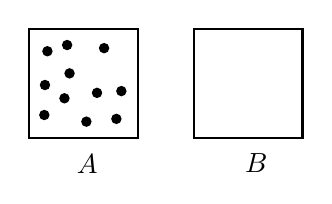
\begin{tikzpicture}[x=0.40,y=0.40,yscale=-1,xscale=1]
%uncomment if require: \path (0,594); %set diagram left start at 0, and has height of 594

%Shape: Square [id:dp774487099896747] 
\draw  [color={rgb, 255:red, 0; green, 0; blue, 0 }  ,draw opacity=1 ] (14.6,103.16) -- (112.94,103.16) -- (112.94,201.5) -- (14.6,201.5) -- cycle ;
%Shape: Square [id:dp025429925890165128] 
\draw   (163.6,103.16) -- (261.94,103.16) -- (261.94,201.5) -- (163.6,201.5) -- cycle ;
%Shape: Circle [id:dp3181813441668684] 
\draw  [fill={rgb, 255:red, 0; green, 0; blue, 0 }  ,fill opacity=1 ] (27.79,123.5) .. controls (27.79,121.46) and (29.45,119.8) .. (31.5,119.8) .. controls (33.54,119.8) and (35.2,121.46) .. (35.2,123.5) .. controls (35.2,125.55) and (33.54,127.21) .. (31.5,127.21) .. controls (29.45,127.21) and (27.79,125.55) .. (27.79,123.5) -- cycle ;
%Shape: Circle [id:dp603908038435023] 
\draw  [fill={rgb, 255:red, 0; green, 0; blue, 0 }  ,fill opacity=1 ] (47.79,143.5) .. controls (47.79,141.46) and (49.45,139.8) .. (51.5,139.8) .. controls (53.54,139.8) and (55.2,141.46) .. (55.2,143.5) .. controls (55.2,145.55) and (53.54,147.21) .. (51.5,147.21) .. controls (49.45,147.21) and (47.79,145.55) .. (47.79,143.5) -- cycle ;
%Shape: Circle [id:dp5952281148881424] 
\draw  [fill={rgb, 255:red, 0; green, 0; blue, 0 }  ,fill opacity=1 ] (24.99,181.1) .. controls (24.99,179.06) and (26.65,177.4) .. (28.7,177.4) .. controls (30.74,177.4) and (32.4,179.06) .. (32.4,181.1) .. controls (32.4,183.15) and (30.74,184.81) .. (28.7,184.81) .. controls (26.65,184.81) and (24.99,183.15) .. (24.99,181.1) -- cycle ;
%Shape: Circle [id:dp8284021424683614] 
\draw  [fill={rgb, 255:red, 0; green, 0; blue, 0 }  ,fill opacity=1 ] (78.99,120.7) .. controls (78.99,118.66) and (80.65,117) .. (82.7,117) .. controls (84.74,117) and (86.4,118.66) .. (86.4,120.7) .. controls (86.4,122.75) and (84.74,124.41) .. (82.7,124.41) .. controls (80.65,124.41) and (78.99,122.75) .. (78.99,120.7) -- cycle ;
%Shape: Circle [id:dp5147293581241896] 
\draw  [fill={rgb, 255:red, 0; green, 0; blue, 0 }  ,fill opacity=1 ] (62.99,187.1) .. controls (62.99,185.06) and (64.65,183.4) .. (66.7,183.4) .. controls (68.74,183.4) and (70.4,185.06) .. (70.4,187.1) .. controls (70.4,189.15) and (68.74,190.81) .. (66.7,190.81) .. controls (64.65,190.81) and (62.99,189.15) .. (62.99,187.1) -- cycle ;
%Shape: Circle [id:dp9005778661722459] 
\draw  [fill={rgb, 255:red, 0; green, 0; blue, 0 }  ,fill opacity=1 ] (94.59,159.5) .. controls (94.59,157.46) and (96.25,155.8) .. (98.3,155.8) .. controls (100.34,155.8) and (102,157.46) .. (102,159.5) .. controls (102,161.55) and (100.34,163.21) .. (98.3,163.21) .. controls (96.25,163.21) and (94.59,161.55) .. (94.59,159.5) -- cycle ;
%Shape: Circle [id:dp1200483422476748] 
\draw  [color={rgb, 255:red, 0; green, 0; blue, 0 }  ,draw opacity=1 ][fill={rgb, 255:red, 0; green, 0; blue, 0 }  ,fill opacity=1 ] (72.59,161.1) .. controls (72.59,159.06) and (74.25,157.4) .. (76.3,157.4) .. controls (78.34,157.4) and (80,159.06) .. (80,161.1) .. controls (80,163.15) and (78.34,164.81) .. (76.3,164.81) .. controls (74.25,164.81) and (72.59,163.15) .. (72.59,161.1) -- cycle ;
%Shape: Circle [id:dp8676035581957091] 
\draw  [fill={rgb, 255:red, 0; green, 0; blue, 0 }  ,fill opacity=1 ] (90.09,184.6) .. controls (90.09,182.56) and (91.75,180.9) .. (93.8,180.9) .. controls (95.84,180.9) and (97.5,182.56) .. (97.5,184.6) .. controls (97.5,186.65) and (95.84,188.31) .. (93.8,188.31) .. controls (91.75,188.31) and (90.09,186.65) .. (90.09,184.6) -- cycle ;
%Shape: Circle [id:dp7565040593219183] 
\draw  [fill={rgb, 255:red, 0; green, 0; blue, 0 }  ,fill opacity=1 ] (45.59,117.9) .. controls (45.59,115.86) and (47.25,114.2) .. (49.3,114.2) .. controls (51.34,114.2) and (53,115.86) .. (53,117.9) .. controls (53,119.95) and (51.34,121.61) .. (49.3,121.61) .. controls (47.25,121.61) and (45.59,119.95) .. (45.59,117.9) -- cycle ;
%Shape: Circle [id:dp5827285696809148] 
\draw  [fill={rgb, 255:red, 0; green, 0; blue, 0 }  ,fill opacity=1 ] (43.19,166) .. controls (43.19,163.96) and (44.85,162.3) .. (46.9,162.3) .. controls (48.94,162.3) and (50.6,163.96) .. (50.6,166) .. controls (50.6,168.05) and (48.94,169.71) .. (46.9,169.71) .. controls (44.85,169.71) and (43.19,168.05) .. (43.19,166) -- cycle ;
%Shape: Circle [id:dp8537532752530581] 
\draw  [fill={rgb, 255:red, 0; green, 0; blue, 0 }  ,fill opacity=1 ] (25.59,154) .. controls (25.59,151.96) and (27.25,150.3) .. (29.3,150.3) .. controls (31.34,150.3) and (33,151.96) .. (33,154) .. controls (33,156.05) and (31.34,157.71) .. (29.3,157.71) .. controls (27.25,157.71) and (25.59,156.05) .. (25.59,154) -- cycle ;

% Text Node
\draw (207.4,213.54) node [anchor=north west][inner sep=0.75pt]    {$\text{B}$};
% Text Node
\draw (55.33,213.87) node [anchor=north west][inner sep=0.75pt]    {$\text{A}$};

\end{tikzpicture}
    \end{figure}

    \begin{itemize}
      \item mean recurrence time: \alert{$2^N$}
      \item for a mole of particles ($N = N_A$), this time is greater than the age of the universe!
    \end{itemize}
  \end{frame}

  \begin{frame}{irreversibility}
    \begin{center}
      \Large \textbf{Explanation of irreversibility}
    \end{center}
    \begin{itemize}
      \item \alert{in principle}, all configurations are reversibile
      \item \alert{in fact}, some configurations are so unlikely that we never see them, statistically
      \item Markov theory allows to quantify reversibility
    \end{itemize}
  \end{frame}
